\documentclass[UTF8]{ctexart}
\usepackage[landscape]{geometry}
\usepackage{color}
\usepackage{ctex}
\usepackage{graphicx}
\usepackage{float}
\usepackage{wrapfig}

\author{Wu Ting}


% \definecolor{MyDarkBlue}{rgb}{0,0.08,0.45}
% \definecolor{yellow}{rgb}{0.99,0.99,0.70}
% \definecolor{myback}{RGB}{255,255,240}
% \definecolor{white}{rgb}{1.0,1.0,1.0}                                         
% \definecolor{red}{RGB}{149,0,64}
% \definecolor{black}{RGB}{0,0,0}
% \definecolor{Silver}{RGB}{192,192,192}
% \pagecolor{Silver}



    
\begin{document}

% 学校和学院校徽
\begin{figure}[H]
    \vspace*{-40pt}
    \flushleft
\includegraphics[scale = 0.9]{szucsselogo}
    \vspace*{-70pt}
    \flushright
\includegraphics[scale = 0.15]{b57}
\end{figure}

\begin{flushleft}
    
    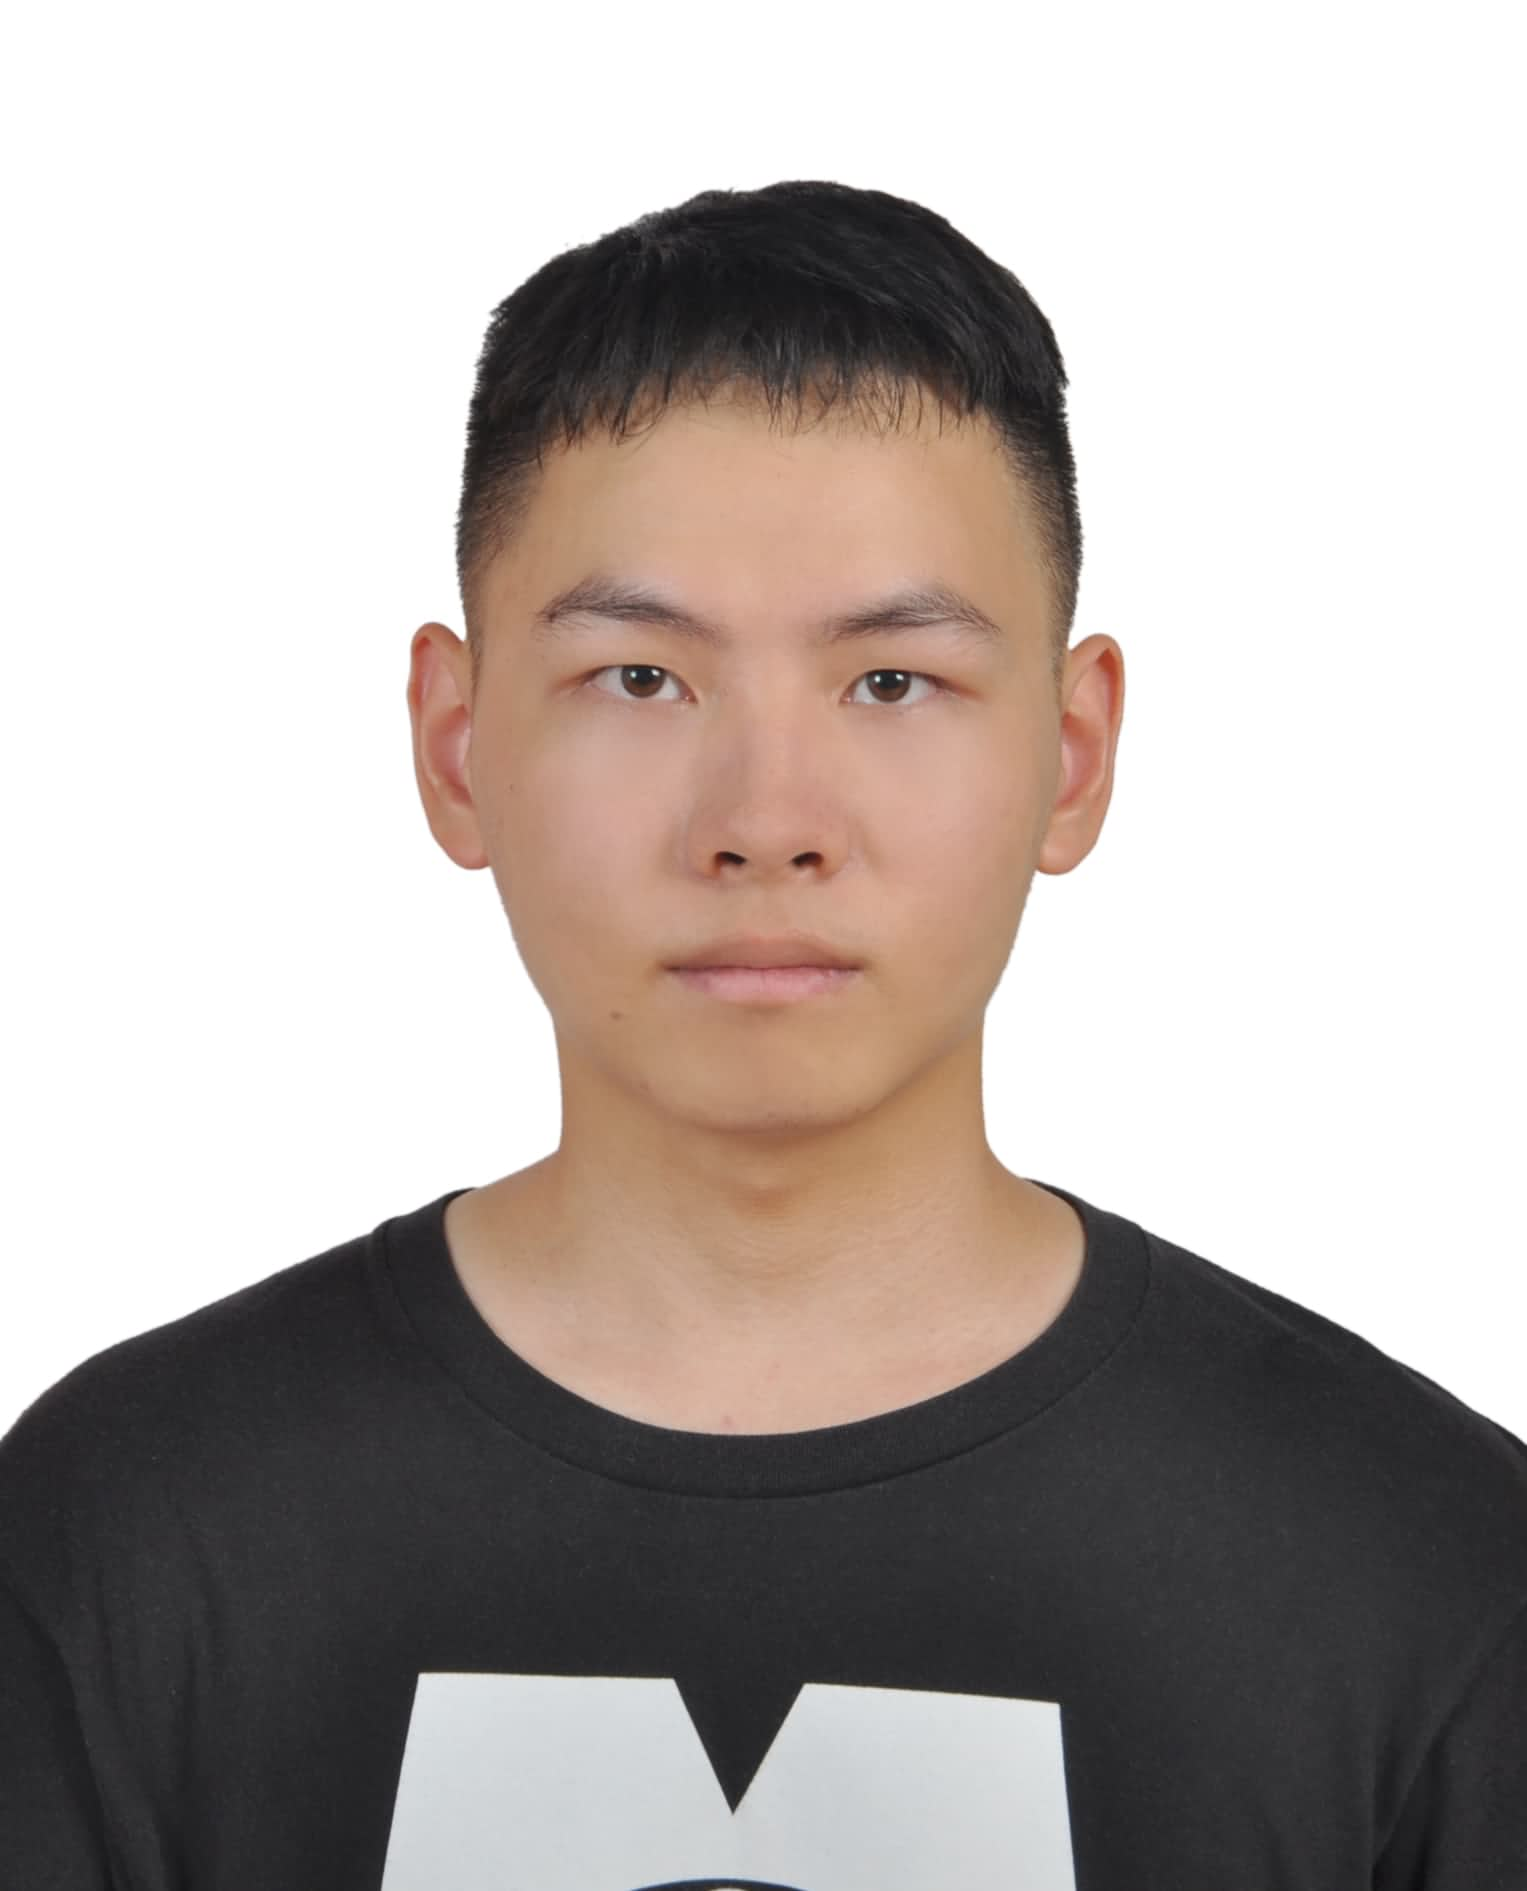
\includegraphics[scale = 0.06]{me}

    \LARGE{\textbf{Wu Ting}}

    \LARGE{\textbf{吴艇}}
    \textsl{(ID:2020281061)}
    
\end{flushleft}

\begin{flushright}
    \vspace*{-150pt}
    \Large{\textbf{email: 1378006836@qq.com/}}

    \Large{\textbf{2020281061@email.szu.cn}}

    \Large{\textbf{hobit: coding,running,traveling}}  
    
    \Large{\textbf{major: Computer Science and Technology}}
  
\end{flushright}

\begin{flushleft}
    \vspace*{90pt}
    \Large{Wu Ting is a student who entered Shenzhen University in 2020.
     His previous major was Electronic and Information Engineering. 
     Last semester, he changed his major to Computer Science and Technology.
     After the college entrance examination last year, he traveled to Shanghai on his own for four days.
     He traveled with his friends to Yunnan during the summer vacation this year. 
     He loves sports, especially running, which can relax his body and mind.
     Last year, He learned front-end in the club, gained a lot of knowledge and made some friends at the same time.
     }
\end{flushleft}


\end{document}